\documentclass[amsmath,superscriptaddress,showpacs,aps,prl,twocolumn]{revtex4-1}
\usepackage[colorlinks,linkcolor=blue,anchorcolor=blue,citecolor=blue,urlcolor=blue]{hyperref}
\usepackage{amsmath}
\usepackage{amssymb}
\usepackage{graphicx}
\usepackage{color}
\usepackage{bm}

\begin{document}
\title{Itinerant topological magnons in Haldane Hubbard model with a nearly-flat electron band}
\author{Zhao-Long Gu}
\affiliation{National Laboratory of Solid State Microstructures and Department of Physics, Nanjing University, Nanjing 210093, China}
\author{Zhao-Yang Dong}
\affiliation{Department of Applied Physics, Nanjing University of Science and Technology, Nanjing 210094, China.}
\affiliation{National Laboratory of Solid State Microstructures and Department of Physics, Nanjing University, Nanjing 210093, China}
\author{Shun-Li Yu}
\affiliation{National Laboratory of Solid State Microstructures and Department of Physics, Nanjing University, Nanjing 210093, China}
\affiliation{Collaborative Innovation Center of Advanced Microstructures, Nanjing University, Nanjing 210093, China}
\author{Jian-Xin Li}
\email[]{jxli@nju.edu.cn}
\affiliation{National Laboratory of Solid State Microstructures and Department of Physics, Nanjing University, Nanjing 210093, China}
\affiliation{Collaborative Innovation Center of Advanced Microstructures, Nanjing University, Nanjing 210093, China}
\date{\today}

\begin{abstract}

\par We propose the first theoretical realization of two dimensional itinerant topological magnons. The microscopic model is the quarter filled spinful Haldane-Hubbard model with a nearly-flat electron band. By using the numerical exact diagonalization method with a projection onto this band, we obtain the spin wave excitations over the itinerant ferromagnetic ground state. The spectra exhibit Dirac magnons in the flatband limit with AB sublattice symmetric Hubbard interactions. Remarkably, although the sublattice Hubbard imbalance opens a trivial gap of the Dirac magnons, the nonflatness of the electron band induces a topological one of the magnon bands. Consistent with the bulk-edge correspondence, there always exist in-gap magnon states on magnetic domain walls. Furthermore, we derive an effective model to describe the itinerant spin wave excitations based on the so-called ``flatband sublattice particle-hole bases''. In the framework of first-order perturbation theory, we elaborate that the generation of the topological magnons can be attributed to the well-known ``mass inversion mechanism''.

\end{abstract}

\maketitle

\par Band structures with nontrivial topology reside at the center of a substantial number of topological phenomena in condensed matter physics \cite{Hasan_RMP2010,Qi_RMP2011,Bansil_RMP2016}. It was proposed in a pioneering work by Haldane \cite{Haldane_PRL1988} that a spinless fermionic model on a honeycomb lattice bears energy bands with nonzero Chern numbers \cite{Thouless_PRL1982,Simon_PRL1983} in the absence of external magnetic fields. In this model, the nonzero Chern number arises from the mechanism that the mass terms of the chirality-opposite lattice Dirac fermions at two isolated points in the first Brillouin zone (FBZ) have different signs. Microscopically, this so-called ``mass inversion mechanism'' is realized by the introduction to the model of a complex next-nearest-neighbor hopping that breaks the time-reversal symmetry. Similar mechanism also applies to other fermionic systems with nontrivial topological bands belonging to different symmetry classes \cite{Kane_PRL2005}.

\par Topological band systems exhibit fascinating physics beyond the traditional Landau paradigm \cite{Chiu_RMP2016,Zeng_B2019}. They cannot be distinguished from trivial ones by local order parameters, but are characterized by nonzero bulk topological indices and featured by gapless edges states on open boundaries \cite{Laughlin_PRB1981,Halperin_PRB1982,Kane_PRL2005a,Bernevig_S2006,Yu_PRL2011,Li_PRB2016,Liu_NJP2017}. The physics of topological bands can be enriched by the presence of strong Coulomb interactions between electrons \cite{Hohenadler_JPCM2013,Wen_RMP2017,Rachel_RPP2018}, especially when the electron bands are nearly flat so that interaction effects are highly enhanced \cite{Neupert_PS2015}. In fractionally-filled strongly-correlated nearly-flat topological bands, more intriguing topological phases of matter, such as fractional Chern insulators \cite{Tang_PRL2011,Wang_PRB2011,Sun_PRL2011,Wang_PRL2011,Neupert_PRL2011,Sheng_NC2011,Regnault_PRX2011} and fractional topological insulators \cite{Neupert_PRB2011}, can be stabilized even at high temperatures. It is noted that previous studies on such systems mainly focus on the charge degree of freedom of electrons. The physics related to the quantum spins that constitute the other fundamental degree of freedom of electrons, has been much less investigated. In most works that consider spinful electron models, the only many-body physics involved with electron spins is the itinerant ferromagnetism \cite{Tasaki_PRL1992,Mielke_PLA1993,Mielke_CMP1993} in the ground state, which is taken as a prerequisite of possible fractional Chern insulators \cite{Tang_PRL2011,Wang_PRB2011,Sun_PRL2011} or integer quantum Hall insulators \cite{Neupert_PRL2012}. The researches \cite{Doretto_PRB2015,Su_PRB2019} on the spin excitations over the ferromagnetic ground state, which can uncover new physics of strongly-correlated nearly-flat topological bands, are still far from sufficient.

\par Interesting clues about the new physics revealed by spin excitations in interacting nearly-flat topological bands come from the community of quantum magnetism. In fact, collective spin excitations over magnetically ordered ground state also exhibit band structures, therefore, exotic magnon excitations with nontrivial band topology are expected to emerge in quantum magnets. Indeed, recently, in a number of local spin materials mostly with Dzyaloshinskii-Moriya (DM) interactions \cite{Dzyaloshinsky_JPCS1958,Moriya_PR1960}, topological magnons have been verified to exist both theoretically \cite{Zhang_PRB2013,Owerre_JPCM2016,Li_NC2016,Mook_PRL2016,Laurell_PRL2017} and experimentally \cite{Onose_S2010,Chisnell_PRL2015,Yao_NP2018,Bao_NC2018}. In such models the magnon excitations are well understood as free bosons in the framework of linear spin wave theory (LSWT), with the DM term acting as the vector potential for the propagation of magnons. However, in the case of itinerant magnets, LSWT fails due to the lack of exact one local electron spin per physical site. The absence of an analytical effective model describing the spin wave excitations makes the investigations on itinerant topological magnons quite arduous \cite{Su_PRB2018}.

\par In this letter, we propose the first theoretical realization of two dimensional itinerant topological magnons and derive an effective model capturing the collective spin excitations to explain the underlying mechanism leading to the nontrivial magnonic topology. The microscopic model is the quarter filled spinful Haldane-Hubbard model with a nearly-flat electron band. By using the numerical exact diagonalization method with a projection onto this electron band, we obtain the spin wave excitations over the itinerant ferromagnetic ground state. The spectra host Dirac magnons in the flatband limit when the AB sublattice Hubbard interactions take on equal values. Remarkably, the nonflatness of the electron band can induce a topological gap of the Dirac magnons, leading to an acoustic magnon band with a nonzero Chern number. Then after the imbalance of the AB sublattice Hubbard interactions is turned on, the magnon gap can be closed and reopened, accompanied by the Chern number of the magnon band changing from nonzero to zero. Besides, with a tuning of the next-nearest-neighbor hopping amplitude, the Chern number of the magnon band can be altered from $+1$ to $-1$, while the topology of the electron band keeps unchanged. Consistent with the bulk-edge correspondence, there always exist in-gap magnon states on magnetic domain walls. Furthermore, based on the so-called ``flatband sublattice particle-hole bases'', we derive an effective model to describe the itinerant spin wave excitations. In the framework of first-order perturbation theory, we elaborate that the generation of the topological magnons can be attributed to the well-known ``mass inversion mechanism''.

\begin{figure}
\centering
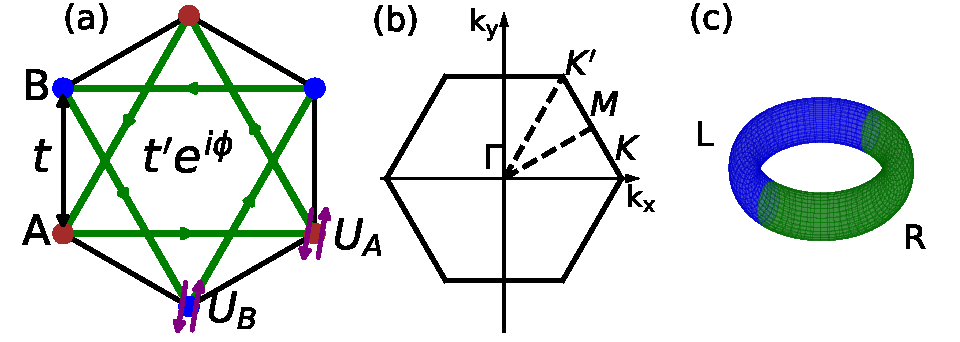
\includegraphics[width=0.48\textwidth]{lattice}
\caption{(color online). (a) Schematic illustration of the Haldane-Hubbard model on honeycomb lattice. A and B denote the two inequivalent sites within a unitcell. The real nearest-neighbor hopping amplitude $t$, the complex next-nearest-neighbor hopping amplitude $t^\prime e^{i\phi}$, and the Hubbard interactions $U_A$ and $U_B$ are also shown. (b) First Brillouin zone of the honeycomb lattice. (c) An illustration of the domain wall geometry.}
\label{lattice}
\end{figure}

\par The Haldane Hubbard model is written as $\hat{H}=\hat{H}_0+\hat{H}_U$ as shown in Fig. \ref{lattice}(a), where $\hat{H}_0$ is the spinful version of the Haldane model on the honeycomb lattice \cite{Haldane_PRL1988},
\begin{equation}\label{H0}
\hat{H}_0=t\sum_{\langle ij\rangle\sigma}c^{\dagger}_{i\sigma}c_{j\sigma}+t'\sum_{\langle\langle ij\rangle\rangle\sigma}e^{\phi_{ij}}c^{\dagger}_{i\sigma}c_{j\sigma}
\end{equation}
and $\hat{H}_U$ is the Hubbard interaction,
\begin{equation}\label{HU}
\hat{H}_U=U\sum_i n_{i\uparrow}n_{i\downarrow}
\end{equation}
Here, $\langle ij\rangle$ and $\langle\langle ij\rangle\rangle$ denote the nearest-neighbor (NN) and next-nearest-neighbor (NNN) bonds, respectively. $\phi_{ij}=\pm\phi$ is the phase of NNN electron hopping with the sign given by the solid green arrows in Fig. \ref{lattice}(a). Others are in standard notation.

\par The free part of the Hamiltonian in the momentum space can be written as $\hat{H}_0=\sum_{\mathbf{k}\sigma}\psi^{\dagger}_{\mathbf{k}\sigma}H_0(\mathbf{k})\psi_{\mathbf{k}\sigma}$. Here, $\psi^{\dagger}_{\mathbf{k}\sigma}=(c^{\dagger}_{A\mathbf{k}\sigma},c^{\dagger}_{B\mathbf{k}\sigma})$, and $H_0(\mathbf{k})=\sum_{\alpha=0,x,y,z}h_\alpha(\mathbf{k})\tau^\alpha$, with $\tau^\alpha$ ($\alpha=0,x,y,z$) the identity matrix and the three Pauli matrices in the sublattice space. Note that $H_0(\mathbf{k})$ is independent of $\sigma$ due to the SU(2) spin rotation symmetry of the model. When $t^\prime=0$, $h_0(\mathbf{k})=h_z(\mathbf{k})=0$, in the FBZ of the honeycomb lattice [see Fig. \ref{lattice}(b)], there exist two Dirac points of the electron band with opposite chiralities at $K/K^\prime$ points. When $t^\prime\ne0$, the Dirac points open gaps, with $h_z(\mathbf{k})\tau^z$ being the mass term. It can be seen that $h_z(K)$ and $h_z(K^\prime)$ have different signs \cite{Haldane_PRL1988}. Therefore, the Chern numbers of the two isolated massive Dirac points do not cancel each other but add up to a nonzero integer \cite{Rachel_RPP2018}. As a consequence, the free electron band for every spin component acquires a nonzero Chern number. More details on this so-called ``mass inversion mechanism'' can be found in the supplement material.

\par With a proper tuning of the amplitude $t^\prime$ and phase $\phi$ of the NNN hopping, the lower electron band of $\hat{H}_0$ can be quite flat. The flatness ratio $\Delta/W$, which is defined as the ratio of the gap $\Delta$ between the two free electron bands to the bandwidth $W$ of the lower one, takes its maximum ($\sim7$) when $\cos\phi=t/4t^\prime=3\sqrt{3/43}$ ($t^\prime/t\simeq0.3155, \phi\simeq0.656$) \cite{Neupert_PRL2011}. The half-filled Haldane-Hubbard model with $\phi=\pi/2$ has been extensively studied before \cite{He_PRB2011a,Maciejko_PRB2013,Zheng_PRB2015,Hickey_PRL2016,Wu_PRB2016,Vanhala_PRL2016,Imriska_PRB2016,Giuliani_PRB2016,Garcia_NJP2018,Gu_NJP2019}. In this letter, we consider the quarter-filled case with a nearly-flat lower electron band. It is well-known that the ground state of such a system is the spin fully polarized ferromagnetic state $|\text{FM}\rangle\equiv\prod_{\mathbf{k}\in\text{FBZ}}d^\dagger_{\mathbf{k}\uparrow}|0\rangle$ when the Hubbard interactions exceed a critical value \cite{Tasaki_PRL1994,Su_PRB2019}. Here, $|0\rangle$ is the electron vacuum, and $d^\dagger_{\mathbf{k}\uparrow}$ creates a spin-up electron with a momentum $\mathbf{k}$ in the lower electron band. The parameter space is restricted to the region where $\Delta$ is larger than both $U_A$ and $U_B$, so that the physics is dominated by the degrees of freedom of this lower band and the whole Hamiltonian $H$ can be projected onto it, as is common in the community of correlated nearly-flat topological bands \cite{Neupert_PRL2011,Regnault_PRX2011,Neupert_PRB2011,Neupert_PRL2012,Su_PRB2019}. Thus, a basis $|\mathbf{k}_i\rangle_\mathbf{q}$ of the spin-1 excitations with a center-of-mass momentum $\mathbf{q}$ over the $|\text{FM}\rangle$ state can be written as $|\mathbf{k}_i\rangle_\mathbf{q}=d^\dagger_{\mathbf{k}_i-\mathbf{q}\downarrow}d_{\mathbf{k}_i\uparrow}|\text{FM}\rangle$. The matrix element of the projected Hamiltonian on this set of bases is
\begin{equation}\label{PHP}
_\mathbf{q}\langle\mathbf{k}_j|P^\dagger HP|\mathbf{k}_i\rangle_\mathbf{q}=\left[M_{i}^1(\mathbf{q})+M_{i}^2(\mathbf{q})\right]\delta_{\mathbf{k}_j,\mathbf{k}_i}-M_{ji}^3(\mathbf{q})
\end{equation}
where, $P$ is the projector onto the lower band, and
\begin{eqnarray}
M_{i}^1(\mathbf{q}) &=& \varepsilon_d(\mathbf{k}_i-\mathbf{q})-\varepsilon_d(\mathbf{k}_i), \label{M1}\\
M_{i}^2(\mathbf{q}) &=& \frac{1}{N}\sum_{a=A,B}U_a\sum_{\mathbf{p}}\left|\mu_{a\mathbf{p}\uparrow}\right|^2\left|\mu_{a\mathbf{k}_{i}-\mathbf{q}\downarrow}\right|^2, \label{M2}\\
M_{ji}^3(\mathbf{q}) &=& \frac{1}{N}\sum_{a=A,B}U_a
\mu^{\ast}_{a\mathbf{k}_i-\mathbf{q}\downarrow}\mu_{a\mathbf{k}_{i}\uparrow}\mu_{a\mathbf{k}_j-\mathbf{q}\downarrow}\mu^{\ast}_{a\mathbf{k}_{j}\uparrow}. \label{M3}
\end{eqnarray}
Here, $N$ is the number of momenta in the FBZ, $\varepsilon_d(\mathbf{k})$ is the dispersion of the lower electron band with the momentum $\mathbf{k}$, and $\mu_{a\mathbf{k}\sigma}$ ($a=A,B$ and $\sigma=\uparrow,\downarrow$) is the probability amplitude of sublattice $a$ that contributes to the lower band $d_{\mathbf{k}\sigma}=\sum_{a=A,B}\mu_{a\mathbf{k}\sigma}c_{a\mathbf{k}\sigma}$ [i.e. $\left(\mu_{A\mathbf{k}\sigma},\mu_{B\mathbf{k}\sigma}\right)^T$ is the eigenvector corresponding to the lower band of $H_0(\mathbf{k})$], such that $P^\dagger c_{a\mathbf{k}\sigma}P=\mu^\ast_{a\mathbf{k}\sigma}d$. It can be seen \cite{Su_PRB2018,Su_PRB2019} that with a projection onto the lower electron band, the dimension of the total Hilbert space of spin-1 excitations scales linearly with respect to the system size, which is in sharp contrast to the exponential dependency in a usual exact diagonalization method. This enables us to access a much larger system. In the following, all the bulk spectra are obtained with a numerical diagonalization of Eq. (\ref{PHP}) with $N=60\times60$.

\begin{figure}
\centering
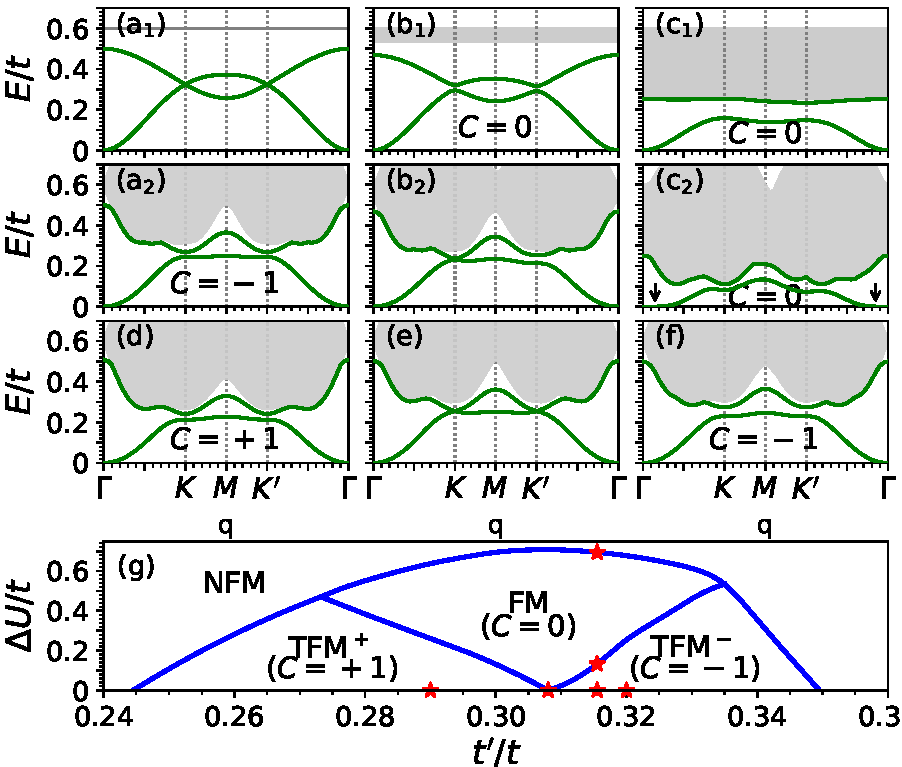
\includegraphics[width=0.48\textwidth]{bulkresult}
\caption{(color online). (a)-(f): Spin-1 excitation spectra of the $1/4$ filled Haldane-Hubbard model with (a) $t^\prime=0.3155$, $U_B=1.2$, (b) $t^\prime=0.3155$, $U_B=1.068$, (c) $t^\prime=0.3155$, $U_B=0.506$, (d) $t^\prime=0.29$, $U_B=1.2$, (e) $t^\prime=0.308$, $U_B=1.2$, (f) $t^\prime=0.32$, $U_B=1.2$. (a$_1$)-(c$_1$): in the flatband limit. (a$_2$)-(c$_2$) and (d)-(f): when the dispersion of the lower electron band is considered. (g) Phase diagram of the $1/4$ filled Haldane-Hubbard model in the $\Delta U(\equiv U_A-U_B)-t^\prime$ parameter space. The red stars mark the parameters used in (a)-(f). Other parameters are fixed at $t=1.0$, $\phi=0.656$, $U_A=1.2$.}
\label{bulkresult}
\end{figure}

\par Now let's turn to the numerical results. We begin with the spin-1 excitation spectra of the model in the flatband limit with symmetric sublattice Hubbard interactions, which are obtained by ignoring the dispersion of the lower electron band (the $M_i^1(\mathbf{q})$ term) and setting $U_A=U_B$ in Eq. (\ref{PHP}). This is also the starting point of our effective model to describe the itinerant spin waves, which will be discussed later. In Fig. \ref{bulkresult}(a$_1$), a result of this case is shown, with $U_A=U_B=1.2t$, $t^\prime=0.3155t$, $\phi=0.656$. The spin-1 excitation spectra consist of two parts: the low-lying spin waves labeled by the green lines contain two branches of well-defined magnon bands, and the high-energy Stoner continuum labeled by the grey region is a horizontal line at $U/2$. The most notable feature of the spin wave excitations is the existence of Dirac (two-fold degenerate) points at $K$/$K^\prime$ in the FBZ.

\par The above magnon Dirac points in the flatband limit with symmetric Hubbard interactions can be gapped by the introduction of the Hubbard imbalance as well as the nonflatness of the lower electron band. As shown in Figs. \ref{bulkresult}(b$_1$)-(c$_1$), the Dirac magnons open gaps at $K$/$K^\prime$ points when only sublattice Hubbard imbalance is added, leading to topological trivial magnon bands in that the Chern number of the acoustic (lower) branch is zero. Remarkably, the magnon gap induced by the nonflatness of the lower electron band, as is shown in Fig. \ref{bulkresult}(a$_2$), is topologically nontrivial since the Chern number of the acoustic magnon band at this time is $-1$. Intriguingly, these two kind of magnon gaps are competitive to each other: as is shown in Figs. \ref{bulkresult}(b$_2$)-(c$_2$), the increase of the Hubbard imbalance can close the topological gap resulted from the nonflatness of the lower electron band, and reopen a trivial one. We want to remark that critical values of Hubbard interactions are needed to maintain the ground state ferromagnetically ordered when the dispersion of the lower electron band is considered \cite{Tasaki_PRL1994,Su_PRB2019}. As indicated by the black arrows in Fig. \ref{bulkresult}(c$_2$), negative spin-1 excitation spectra in the acoustic branch is about to develop at some points between $\Gamma$ and $K/K^\prime$, which will result in the destabilization of the ferromagnetic ground state \cite{Su_PRB2019}. Another interesting observation is that the Chern number of the acoustic magnon band can be altered from $+1$ to $-1$ with a tuning of the NNN electron hopping amplitude, as is shown in Figs. \ref{bulkresult}(d)-(f), although the topology of the electron bands keep unchanged during this process. Besides, we also find that the Chern number of the magnon band changes its sign if we revert the NNN electron hopping phase $\phi$.

\par The above discussion can be summarized by the phase diagram shown in Fig. \ref{bulkresult}(g). In the $\Delta U-t^\prime$ parameter space, where $\Delta U\equiv U_A-U_B$, we find one nonferromagnetic (NFM) phase and three ferromagnetic phases with different magnon band topologies, i.e. the trivial ferromagnetic phase (FM) with zero Chern number, and the two topological ferromagnetic phases (TFM$^+$ and TFM$^-$) with $\pm1$ Chern number, respectively.

\begin{figure}
\centering
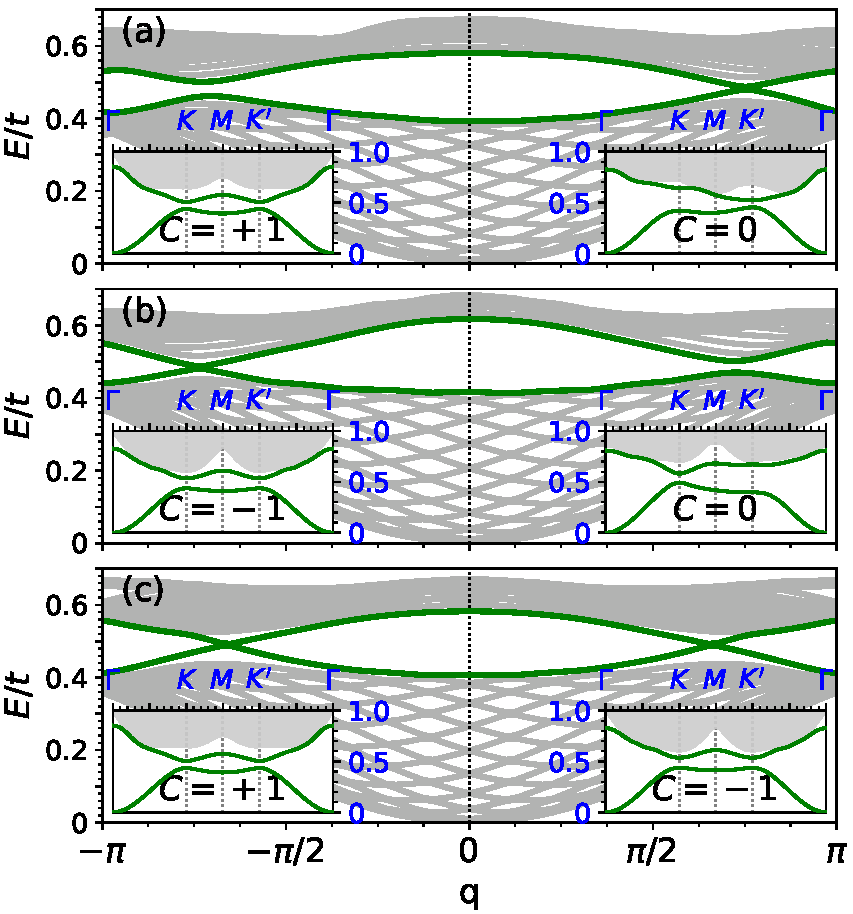
\includegraphics[width=0.48\textwidth]{domainwallspectra}
\caption{(color online). Spin-1 excitation spectra of the $1/4$ filled Haldane-Hubbard model on magnetic domain walls with (a) $t^{\prime L}=t^{\prime R}=0.28$, $U^L_A=2.0$, $U^L_B=2.0$, $U^R_A=2.7$, $U^R_B=1.7$, (b) $t^{\prime L}=t^{\prime R}=0.33$, $U^L_A=2.0$, $U^L_B=2.0$, $U^R_A=2.7$, $U^R_B=1.7$, (c) $t^{\prime L}=0.28$, $t^{\prime R}=0.33$, $U^L_A=U^L_B=U^R_A=U^R_B=2.0$. Other parameters are fixed at $t=1.0$, $
\phi=0.656$. Insets show the corresponding bulk spin-1 excitation spectra of the left and right halves of the domain wall system.}
\label{domainwallspectra}
\end{figure}

\par According to the bulk-edge correspondence, the topological magnon band in the TFM$^+$ and TFM$^-$ phases should lead to localized in-gap magnon modes when the system is subject to open boundary conditions. However, the electron band is also topological, and the electron edge states would destabilize the ferromagnetic order in the ground state because they go across the whole electron gap between the upper and lower electron band so that the spin fully polarized state is no more energetically favorable. As an alternative, we explore the in-gap magnon states on magnetic domain walls, as illustrated in Fig. \ref{lattice}(c). In such geometry, the system still assumes periodic boundary conditions on both directions whereas along one direction, say along the x direction, it is composed of two halves which take on different model parameters such that the electron band topologies are the same but the magnon band topologies are different. Another difficulty is due to the numerics. The computation cost scales with $N_x^2\times N_y$ because of the lack of momentum conservation along the x direction, where $N_x$ and $N_y$ are the number of unit cells in the domain wall geometry along x and y directions, respectively. This restricts $N_x$ down to about a dozen in our calculations. Yet as can be seen in Figs. \ref{bulkresult}(a)-(f), the magnon band gap is quite small, making the numerical verification of the in-gap domain wall magnon states rather difficult. To resolve this, we artificially extend the phase diagram in Fig. \ref{bulkresult}(g) to a parameter space with much larger $U_A$ and $U_B$ and hence the magnon band gap. Although physically with such parameters the projection onto the lower electron band does not apply any more, it is suitable for the illustration of a numerical check for the existence of in-gap magnon domain wall states. In Fig. \ref{domainwallspectra}(a)-(c), with larger Hubbard interactions than those in Fig. \ref{bulkresult}, the magnon spectra on TFM$^+$-FM, TFM$^-$-FM and TFM$^+$-TFM$^-$ domain walls are shown, respectively. The insets are the corresponding bulk spin-1 excitation spectra of the two halves of the domain wall system. Clearly, the number of chiral in-gap magnon modes equals the Chern number difference between the two halves for all three cases, which is expected by the bulk-edge correspondence exactly.

\begin{figure}
\centering
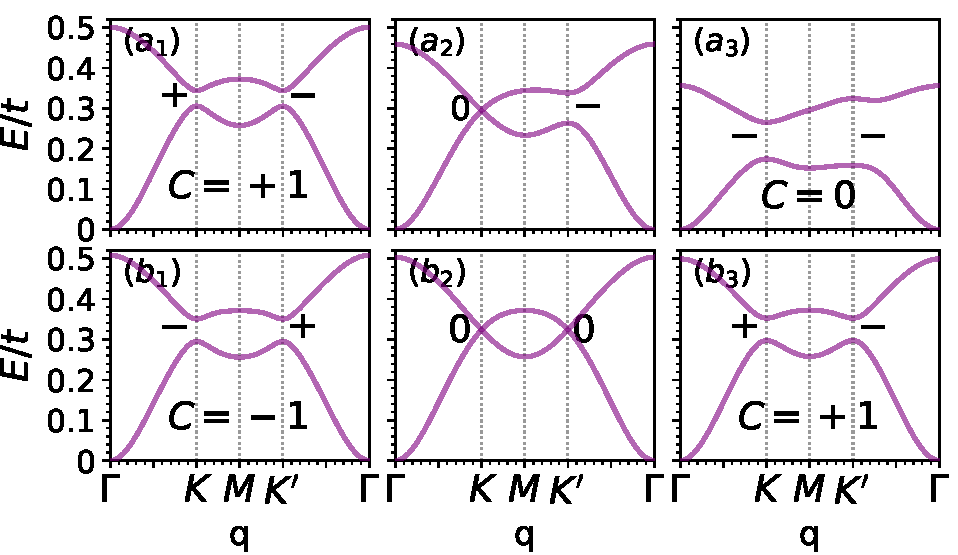
\includegraphics[width=0.48\textwidth]{effectivespectra}
\caption{(color online). Dispersion relations of spin waves obtained by first-order perturbation theory applied to the effective model with (a$_1$) $t^\prime=0.3155$, $U_B=1.2$, (a$_2$) $t^\prime=0.3155$, $U_B=1.0$, (a$_3$) $t^\prime=0.3155$, $U_B=0.506$, (b$_1$) $t^\prime=0.29$, $U_B=1.2$, (b$_2$) $t^\prime=0.3055$, $U_B=1.2$, (b$_3$) $t^\prime=0.32$, $U_B=1.2$. Other parameters are fixed at $t=1.0$, $\phi=0.656$, $U_A=1.2$. The $+$/$-$ marks denote the signs of the mass terms at $K$($K^\prime$) points and $0$ indicate that the mass term is zero.}
\label{effectivespectra}
\end{figure}

\par Different from local spin models where LSWT provides a comprehensive understanding of the magnon band topology, previous researches \cite{Su_PRB2018} on the itinerant spin waves are held back by the lack of an effective theory parallel to the LSWT. Here we propose a general framework which can effectively describe the itinerant magnon excitations over the ferromagnetic ground state in nearly-flat electron bands, based on which the nontrivial magnon band topology can be explained by the ``mass inversion mechanism''. Let's start with the model in the flatband limit with symmetric sublattice Hubbard interactions again. It can be proved (see supplement material) that $M^2_i(\mathbf{q})=U/2$ when $U_A=U_B=U$. The most insightful observation is that $M^3_{ji}(\mathbf{q})$ can be decomposed as the sum of the direct product between the same vectors: $M^3_{ji}(\mathbf{q})=-\sum_{a=A,B}|v^a_i(\mathbf{q})\rangle\langle v^a_j(\mathbf{q})|$, where $|v^a_i(\mathbf{q})\rangle\equiv\sqrt{\frac{U_a}{N}}\mu^{\ast}_{a\mathbf{k}_i-\mathbf{q}\downarrow}\mu_{a\mathbf{k}_{i}\uparrow}$. Each component of the vector $|v^a(\mathbf{q})\rangle$ is the probability amplitude to create a spin-1 particle-hole excitation in the lower electron band within a certain sublattice $a$, thus, we call this vector the ``flatband sublattice particle-hole vector''. It can be shown that in the space spanned by $|v^A(\mathbf{q})\rangle$ and $|v^B(\mathbf{q})\rangle$, Eq. (\ref{PHP}) reduces to a $2\times2$ matrix in the flatband limit with symmetric sublattice Hubbard interactions:
\begin{equation}\label{effective}
M^\text{Flat}_{ab}(\mathbf{q})=\frac{U}{2}\delta_{ab}-\sum_i\langle v_i^a(\mathbf{q})|v_i^b(\mathbf{q})\rangle.
\end{equation}
Note that the off-diagonal matrix element exists because $|v^A(\mathbf{q})\rangle$ and $|v^B(\mathbf{q})\rangle$ are not orthogonal in general. Around $K/K^\prime$ points in the FBZ, $M^\text{Flat}(\mathbf{q})$ behaves as massless-Dirac-like Hamiltonians with opposite chiralities (see supplement material). When the dispersion of the lower electron band or the Hubbard imbalance are considered, these terms can be treated as perturbations to Eq. (\ref{effective}) and again we obtain $2\times2$ effective Hamiltonians up to the first order approximation. Remarkably, we find that at $K/K^\prime$ points in the FBZ, they act exactly as the mass terms of the Dirac magnons. By use of this framework, in Figs. \ref{effectivespectra}(a)-(b), we plot the effective spectra of the magnons parallel to the cases shown in Figs. \ref{bulkresult}(a$_2$)-(c$_2$) and Figs. \ref{bulkresult}(d)-(f). The sign of the mass term induced by the nonflatness of the lower electron band or Hubbard imbalance is also indicated by $+$/$-$. Apparently, all topological phases with magnon bands hosting nonzero Chern numbers have the opposite-signed mass term while trivial phases have the same-signed mass term. More details can be found in the supplement material.

\par In summary, we report the first theoretical proposal of two dimensional itinerant topological magnons by numerical and analytical investigations on the quarter- filled Haldane Hubbard model with a nearly flat electron band. We find Dirac magnons in the flatband limit with symmetric sublattice Hubbard interactions. Although the Hubbard imbalance opens trivial gaps for the Dirac magnons, the magnon gap induced by the nonflatness of the lower electron band is topological. Consistent with the bulk-edge correspondence, there always exist in-gap magnon states on magnetic domain walls. Based on the ``flatband sublattice particle-hole bases'', we propose a general framework to effectively describe the itinerant spin wave excitations and attribute the nontrivial magnon band topology to the ``mass inversion mechanism''.

\begin{acknowledgments}
\par This work was supported by the National Natural Science Foundation of China (11774152) and National Key Projects for Research and Development of China (Grant No. 2016YFA0300401).
\end{acknowledgments}

\bibliography{reference}

\widetext
\newpage
\appendix
\section{Supplemental Material}

\setcounter{equation}{0}
\setcounter{figure}{0}
\setcounter{table}{0}
\setcounter{section}{0}
\renewcommand{\theequation}{S\arabic{equation}}
\renewcommand{\thesection}{S\arabic{section}}
\renewcommand{\thetable}{S\arabic{table}}
\renewcommand{\thefigure}{S\arabic{figure}}

\section{Haldane model and mass inversion mechanism}
\par The free part $\hat{H}_0$ of the Hamiltonian of the Haldane Hubbard model in the momentum space can be written as $\hat{H}_0=\sum_{\mathbf{k}\sigma}\psi^{\dagger}_{\mathbf{k}\sigma}H_0(\mathbf{k})\psi_{\mathbf{k}\sigma}$, where $\psi^{\dagger}_{\mathbf{k}\sigma}=(c^{\dagger}_{A\mathbf{k}\sigma},c^{\dagger}_{B\mathbf{k}\sigma})$, and
\begin{equation}\label{H0k}
H_0(\mathbf{k})=\sum_{\alpha=0,x,y,z}h_\alpha(\mathbf{k})\tau^\alpha,
\end{equation}
with $\tau^\alpha$ ($\alpha=0,x,y,z$) being the identity matrix and the three Pauli matrices in the sublattice space, and
\begin{eqnarray*}
h_0(\mathbf{k})&=&2t^\prime\cos\phi\sum_{i=1}^3\cos(\mathbf{k}\cdot\mathbf{b_i}), \\
h_1(\mathbf{k})&=&t\sum_{i=1}^3\cos(\mathbf{k}\cdot\mathbf{a}_i), \\
h_2(\mathbf{k})&=&-t\sum_{i=1}^3\sin(\mathbf{k}\cdot\mathbf{a}_i), \\
h_3(\mathbf{k})&=&-2t^\prime\sin\phi\sum_{i=1}^3\sin(\mathbf{k}\cdot\mathbf{b}_i).
\end{eqnarray*}
Here, $\mathbf{a}_1$, $\mathbf{a}_2$ and $\mathbf{a}_3$ are the displacements from a A site to its three NN B sites, defined so that $\mathbf{a}_1\times\mathbf{a}_2$ points to the positive direction of z axis, and $\mathbf{b}_1=\mathbf{a}_2-\mathbf{a}_3$, $\mathbf{b}_2=\mathbf{a}_3-\mathbf{a}_1$, $\mathbf{b}_3=\mathbf{a}_1-\mathbf{a}_2$. Note that due to the SU(2) spin rotation symmetry, $H_0(\mathbf{k})$ is independent of $\sigma$. Therefore, we will omit the spin index in the following in this section. The dispersion relation of the free electron bands reads
\begin{eqnarray*}
E^+(\mathbf{k})&=& h_0(\mathbf{k})+h(\mathbf{k}), \\
E^-(\mathbf{k})&=& h_0(\mathbf{k})-h(\mathbf{k}),
\end{eqnarray*}
where $h(\mathbf{k})=\sqrt{h^2_1(\mathbf{k})+h^2_2(\mathbf{k})+h^2_3(\mathbf{k})}$. The corresponding eigenvectors are
\begin{eqnarray}
\Psi_{E^+}(\mathbf{k})&=& \frac{1}{\sqrt{2h(\mathbf{k})\left[(h(\mathbf{k})+h_3(\mathbf{k})\right]}}
\begin{bmatrix}
h_3(\mathbf{k})+h(\mathbf{k}) \\
h_1(\mathbf{k})+ih_2(\mathbf{k})
\end{bmatrix},
\label{PsaiP}\\
\Psi_{E^-}(\mathbf{k})&=& \frac{1}{\sqrt{2h(\mathbf{k})\left[(h(\mathbf{k})-h_3(\mathbf{k})\right]}}
\begin{bmatrix}
h_3(\mathbf{k})-h(\mathbf{k})\\
h_1(\mathbf{k})+ih_2(\mathbf{k})
\end{bmatrix}\label{PsaiM}.
\end{eqnarray}
The Berry connection $A_i(\mathbf{k})$($i=k_x,k_y$) of the lower electron band is
\begin{equation*}
A_i(\mathbf{k}) = i\langle\Psi_{E^-}(\mathbf{k})|\partial_{k_i}|\Psi_{E^-}(\mathbf{k})\rangle
                         = \frac{-1}{2h\left(h-h_3\right)}\left(h_2\partial_{k_i}h_1-h_1\partial_{k_i}h_2\right),
\end{equation*}
and the corresponding Berry curvature $F(\mathbf{k})$ is
\begin{equation*}
F(\mathbf{k}) = \partial_{k_x}A_{k_x}-\partial_{k_y}A_{k_y}
              = \frac{1}{2h^3}\epsilon_{abc}h_a\partial_{k_x}h_b\partial_{k_y}h_c,
\end{equation*}
where $\epsilon_{abc}$ is the total antisymmetric tensor. When $t^\prime=0$ and hence $h_0(\mathbf{k})=h_3(\mathbf{k})=0$, there are two inequivalent massless Dirac points of the free electron bands at $K/K^\prime=\frac{4\pi}{3}(\pm1,0)$ in the FBZ. Expand Eq. (\ref{H0k}) around $K/K^\prime$ points, i.e. let $\mathbf{k}\rightarrow K/K^\prime+\mathbf{k}$ where the latter $\mathbf{k}$ is small, we find
\begin{eqnarray}
H_0^K(\mathbf{k})          &\simeq& m_0\tau^0+v_F\left(k_x\tau^x+k_y\tau^y\right)-m_z\tau^z, \label{HK1} \\
H_0^{K^\prime}(\mathbf{k}) &\simeq& m_0\tau^0+v_F\left(-k_x\tau^x+k_y\tau^y\right)+m_z\tau^z. \label{HK2}
\end{eqnarray}
Here, $m_0=-3t^\prime\cos\phi$, $v_F=-\frac{\sqrt{3}}{2}t$, and $m_z=3t^\prime\sin\phi$. Clearly, when $t^\prime\ne0$ and $\phi\ne0$, Eqs. (\ref{HK1})-(\ref{HK2}) are massive Dirac Hamiltonians with opposite-signed mass terms (the $\pm m_z\tau^z$ term). Due to the different sign of the $\tau^x$ term, these Dirac Hamiltonians have opposite chiralities as well. Correspondingly, the Berry curvature of the lower electron band around $K/K^\prime$ points becomes
\begin{equation*}
F^K(\mathbf{k})\simeq F^{K^\prime}(\mathbf{k})\simeq-\frac{v_F^2m_z}{2\left[m_z^2+(v_Fk_x)^2+(v_Fk_y)^2\right]^{3/2}}
\end{equation*}
The Chern number $C$ of the lower electron band is the sum of individual contributions $C^{K/K^\prime}$ from the above massive Dirac points:
\begin{equation*}
C^{K/K^\prime}=\frac{1}{2\pi}\int d^2\mathbf{k} F^{K/K^\prime}(\mathbf{k})=-\frac{\text{sign}(m_z)}{2}.
\end{equation*}
Therefore, $C=C^K+C^{K^\prime}=-\text{sign}(m_z)$. When $m_z\ne0$, the Chern number of the lower electron band is $\pm1$ depending on the sign of $m_z$. Following the above derivations, we want to remark that the Chern number of a single massive Dirac point is always $\pm1/2$, whose sign is determined by its chirality as well as the sign of its mass term. With an reversion of its chirality or its mass sign, the Chern number is also reverted. Thus, for a lattice model that hosts two Dirac points with opposite chiralities, a nonzero Chern number of the energy band exists if and only if the sign of the mass term at these two Dirac points are different. This is the so-called ``mass inversion mechanism''.

\section{Details on the effective model describing the spin wave excitations in 1/4 filled Haldane-Hubbard model with a nearly flat electron band}
\par When the lower electron band of the Haldane-Hubbard model is nearly flat by a proper tuning of $t^\prime$ and $\phi$, the low-energy physics is dominated by the degrees of freedom in this band if it is fractionally filled for the parameter space where the Hubbard interactions are smaller than the electron gap between the two free electron bands. Then the Hamiltonian can be projected onto this band. According to Eq. (\ref{PsaiM}), the eigen operator of this band is $d_{\mathbf{k}\sigma}=\mu_{A\mathbf{k}\sigma}c_{A\mathbf{k}\sigma}+\mu_{B\mathbf{k}\sigma}c_{B\mathbf{k}\sigma}$, with
\begin{equation*}
\mu_{A\mathbf{k}\sigma} =  \frac{h_3(\mathbf{k})-h(\mathbf{k})}{\sqrt{2h(\mathbf{k})\left[(h(\mathbf{k})-h_3(\mathbf{k})\right]}}, \;
\mu_{B\mathbf{k}\sigma} =  \frac{h_1(\mathbf{k})+ih_2(\mathbf{k})}{\sqrt{2h(\mathbf{k})\left[(h(\mathbf{k})-h_3(\mathbf{k})\right]}}.
\end{equation*}
For Eq. (\ref{M2}) in the main text, if $U_A=U_B=U$, we have
\begin{equation*}
M^2_i(\mathbf{q})=\frac{U}{N}\sum_{\mathbf{p}}\left|\mu_{A\mathbf{p}\uparrow}\right|^2\left|\mu_{A\mathbf{k}_i-\mathbf{p}\downarrow}\right|^2
                 +\left|\mu_{B\mathbf{p}\uparrow}\right|^2\left|\mu_{B\mathbf{k}_i-\mathbf{p}\downarrow}\right|^2.
\end{equation*}
Note that
\begin{equation*}
\left|\mu_{A\mathbf{p}\sigma}\right|^2 = \frac{1}{2}\left[1-\frac{h_3(\mathbf{p})}{2h(\mathbf{p})}\right],\;
\left|\mu_{B\mathbf{p}\sigma}\right|^2 = \frac{1}{2}\left[1+\frac{h_3(\mathbf{p})}{2h(\mathbf{p})}\right].
\end{equation*}
However, $h_3(-\mathbf{p})=-h_3(\mathbf{p})$ and $h(-\mathbf{p})=h(\mathbf{p})$, thus, $\sum_{\mathbf{p}}h_3(\mathbf{p})/h(\mathbf{p})=0$. Therefore,
\begin{equation*}
M^2_i(\mathbf{q})=\frac{U}{N}\sum_{\mathbf{p}}\frac{1}{2}\left|\mu_{A\mathbf{k}_i-\mathbf{p}\downarrow}\right|^2
                 +\frac{1}{2}\left|\mu_{B\mathbf{k}_i-\mathbf{p}\downarrow}\right|^2
                 =\frac{U}{2}.
\end{equation*}
On the other hand, in terms of the ``flatband sublattice particle-hole vectors'' $|v^a_i(\mathbf{q})\rangle\equiv\sqrt{\frac{U_a}{N}}\mu^{\ast}_{a\mathbf{k}_i-\mathbf{q}\downarrow}\mu_{a\mathbf{k}_{i}\uparrow}$ ($a=A,B$), Eq. (\ref{M3}) can be written as $M^3_{ji}(\mathbf{q})=-\sum_{a=A,B}|v^a_i(\mathbf{q})\rangle\langle v^a_j(\mathbf{q})|$. Clearly, the eigenvectors with nonzero eigenvalues of $M^3(\mathbf{q})$ must be a superposition of vector $|v^A(\mathbf{q})\rangle$ and vector $|v^B(\mathbf{q})\rangle$. In the flatband limit with symmetric sublattice Hubbard interactions, Eq. (\ref{PHP}) reduces to
\begin{equation*}
M^\text{Flat}_{ji}(\mathbf{q})\equiv\left.\left[M^2(\mathbf{q})\delta_{\mathbf{k}_j,\mathbf{k}_i}+M^3_{ji}(\mathbf{q})\right]\right|_{U_A=U_B=U}
=\frac{U}{2}\delta_{\mathbf{k}_j,\mathbf{k}_i}-\sum_{a=A,B}|v^a_i(\mathbf{q})\rangle\langle v^a_j(\mathbf{q})|
\end{equation*}
Therefore, the eigenvectors of $M^\text{Flat}$ superposed by $|v^A(\mathbf{q})\rangle$ and $|v^B(\mathbf{q})\rangle$ correspond to the spin wave excitations and the eigenvectors of $M^\text{Flat}$ with $U/2$ eigenvalues correspond to the Stoner continuum. Thus, the space spanned by $|v^A(\mathbf{q})\rangle$ and $|v^B(\mathbf{q})\rangle$ defines the effective space of the spin wave excitations of $M^\text{Flat}$. In this space, $M^\text{Flat}$ reduces to a $2\times2$ matrix, which is shown by the Eq. (\ref{effective}) in the main text. When the dispersion of the lower electron band or sublattice Hubbard imbalance are considered, these terms can be treated as perturbations to Eq. (\ref{effective}). However, $|v^A(\mathbf{q})\rangle$ and $|v^B(\mathbf{q})\rangle$ are generally not orthonormal, making the evaluation of the matrix elements quite complicated. For simplicity, a set of orthonormalized bases will be used instead, which can be obtained by the standard Gram-Schmidt orthogonalization in linear algebra:
\begin{eqnarray*}
|\hat{v}^1(\mathbf{q})\rangle&=&S_{11}(\mathbf{q})|v^A(\mathbf{q})\rangle+S_{21}(\mathbf{q})|v^B(\mathbf{q})\rangle,\\
|\hat{v}^2(\mathbf{q})\rangle&=&S_{12}(\mathbf{q})|v^A(\mathbf{q})\rangle+S_{22}(\mathbf{q})|v^B(\mathbf{q})\rangle,
\end{eqnarray*}
with
\begin{equation}\label{Schmidt}
S_{11}(\mathbf{q})=\frac{1}{s_1(\mathbf{q})},\;
S_{21}(\mathbf{q})=0,\;
S_{12}(\mathbf{q})=-\frac{s_2(\mathbf{q})}{s_3(\mathbf{q})},\;
S_{22}(\mathbf{q})=\frac{1}{s_3(\mathbf{q})}.
\end{equation}
where $s_1(\mathbf{q})=\text{Norm}(|v^A(\mathbf{q})\rangle)$, $s_2(\mathbf{q})=\langle v^A(\mathbf{q})|v^B(\mathbf{q})\rangle/s_1^2$, and $s_3(\mathbf{q})=\text{Norm}(|v^B(\mathbf{q})\rangle-s_2|v^A(\mathbf{q})\rangle)$. Here $\text{Norm}(|v\rangle)$ is the function to get the norm of a vector $|v\rangle$: $\text{Norm}(|v\rangle)=\sqrt{\langle v|v\rangle}$. By use of the $\{|\hat{v}^1(\mathbf{q})\rangle,|\hat{v}^2(\mathbf{q})\rangle\}$ bases, the spin wave excitations of Eq. (\ref{PHP}) up to the first order perturbation approximation can be described by the following matrix:
\begin{equation}\label{Effective1st}
M^{\text{1st}}_{\alpha\beta}(\mathbf{q})=M^0_{\alpha\beta}(\mathbf{q})+M^\Omega_{\alpha\beta}(\mathbf{q})+M^{dU}_{\alpha\beta}(\mathbf{q}),
\end{equation}
with
\begin{eqnarray}
M^0_{\alpha\beta}(\mathbf{q}) &=& \frac{U_A+U_B}{2}\delta_{\alpha\beta}+\left(\left[S^\dagger(\mathbf{q}) S(\mathbf{q})\right]^{-1}\right)_{\alpha\beta}, \\
M^\Omega_{\alpha\beta}(\mathbf{q}) &=& \sum_i\langle\hat{v}^\alpha_i(\mathbf{q})
                                     |\epsilon_d(\mathbf{k}_i-\mathbf{q})-\epsilon(\mathbf{k}_i)|
                                     \hat{v}^\beta_i(\mathbf{q})\rangle, \\
M^{dU}_{\alpha\beta}(\mathbf{q}) &=& \frac{U_A-U_B}{2N}\sum_{s=A,B}\sum_i(-1)^s\langle\hat{v}^\alpha_i(\mathbf{q})
                                 |\sum_{\mathbf{p}}\left|\mu_{s\mathbf{p}\uparrow}\mu_{s\mathbf{k}_{i}-\mathbf{q}\downarrow}\right|^2|
                                 \hat{v}^\beta_i(\mathbf{q})\rangle,
\end{eqnarray}
where the $S$ matrix is defined by Eq. (\ref{Schmidt}), and $(-1)^A\equiv1$, $(-1)^B\equiv-1$. $M^{\text{1st}}(\mathbf{q})$ is a $2\times2$ Hermitian matrix, therefore, it can be expressed as
\begin{equation}\label{M}
M^{\text{1st}}(\mathbf{q})=\sum_{\alpha=0,x,y,z}m^\alpha(\mathbf{q})\sigma^\alpha
\end{equation}
with $\sigma^\alpha$($\alpha=0,x,y,z$) the identity matrix and the three Pauli matrices in the $\{|\hat{v}^1(\mathbf{q})\rangle,|\hat{v}^2(\mathbf{q})\rangle\}$ space. In theory, with Eqs. (\ref{Schmidt})-(\ref{M}), the analytical expressions for $m^\alpha(\mathbf{q})$ can be obtained. However, these expressions are too complicated to analyze, thus, we will only compute them numerically and study the asymptotic behavior of Eq. (\ref{M}) around the $K/K^\prime$ points, which is enough for the exploration of the topological properties of the magnon bands.
\par (1) When $U_A=U_B=U>0$ and in the flatband limit, we find two massless Dirac-like effective Hamiltonians with opposite chiralities near the $K/K^\prime$ points:
\begin{eqnarray*}
M^{\text{1st}}_K(\mathbf{q})          &\simeq& v_0\sigma^0+v_xq_x\sigma^x+v_yq_y\sigma^y, \\
M^{\text{1st}}_{K^\prime}(\mathbf{q}) &\simeq& v_0\sigma^0+v_xq_x\sigma^x-v_yq_y\sigma^y.
\end{eqnarray*}
where $v_0$, $v_x$ and $v_y$ are some constants dependent on the model parameters.
\par (2) When $U_A=U_B=U>0$ and the dispersion of the lower electron band is considered, we find two massive Dirac-like effective Hamiltonians with opposite chiralities as well as opposite mass terms near the $K/K^\prime$ points:
\begin{eqnarray*}
M^{\text{1st}}_K(\mathbf{q})          &\simeq& v_0^\prime\sigma^0+v_x^\prime q_x\sigma^x+v_y^\prime q_y\sigma^y+v_z\sigma^z, \\
M^{\text{1st}}_{K^\prime}(\mathbf{q}) &\simeq& v_0^\prime\sigma^0+v_x^\prime q_x\sigma^x-v_y^\prime q_y\sigma^y-v_z\sigma^z.
\end{eqnarray*}
where $v_0^\prime$, $v_x^\prime$ and $v_y^\prime$ and $v_z$ are some constants dependent on the model parameters. Note that the fermi velocity of the Dirac magnons are also renormalized by the nonflatness of the lower electron band. In this case, according to the ``mass inversion mechanism'', the magnon band are topological with a nonzero ($\pm1$) Chern number.
\par (3) When $U_A\ne U_B>0$ and in the flatband limit, we find two massive Dirac-like effective Hamiltonians with opposite chiralities but with the same-signed mass terms near the $K/K^\prime$ points:
\begin{eqnarray*}
M^{\text{1st}}_K(\mathbf{q})          &\simeq& v_0^K\sigma^0+v_x^K q_x\sigma^x+v_y^K q_y\sigma^y+v^K_z\sigma^z, \\
M^{\text{1st}}_{K^\prime}(\mathbf{q}) &\simeq& v_0^{K^\prime}\sigma^0+v_x^{K\prime} q_x\sigma^x-v_y^{K\prime} q_y\sigma^y+v_z^{K\prime}\sigma^z.
\end{eqnarray*}
where $v_0^{K/K^\prime}$, $v_x^{K/K^\prime}$, $v_y^{K/K^\prime}$, and $v_z^{K/K^\prime}$ are some constants dependent on the model parameters. Note that at $K$ and $K^\prime$ points, these parameters bear asymmetry in the amplitude but share the same sign. According to the ``mass inversion mechanism'', the magnon band for this case are topologically trivial with zero Chern number.
\par (4) When $U_A\ne U_B>0$ and the dispersion of the lower electron band is considered, we still find two massive Dirac-like effective Hamiltonians with opposite chiralities. But now the signs of the mass terms are dependent on both $\Delta U$ and the nonflatness of the lower electron band. When $\Delta U$ is dominant, the mass terms at $K/K^\prime$ points have the same sign, and the magnon band is trivial while when the nonflatness of the lower electron band is dominant, the mass terms at $K/K^\prime$ points have opposite signs and the magnon band is topological.

\end{document}
